\section{SIMD-nodes}

\TODO{This is very detailed and more of a documentation, rather than an
  explanation of how the SIMD nodes work. This section should be rewritten
  entirely (as per issue \#3).}

All SIMD nodes shares the same instruction set and execute instructions in
parallel. {\tt Word} size is 8 bit. Each SIMD node is fully equipped with
registers, an aritmetic logic unit (ALU), message passing and instruction
handling through the SIMD Node instruction set, which is explained within this
section.

The schematic of a SIMD node is shown in figure
\ref{fig:fpga-simd-arch}. \TODO{Talk around the figure}

\begin{figure}[h]
  \centering
 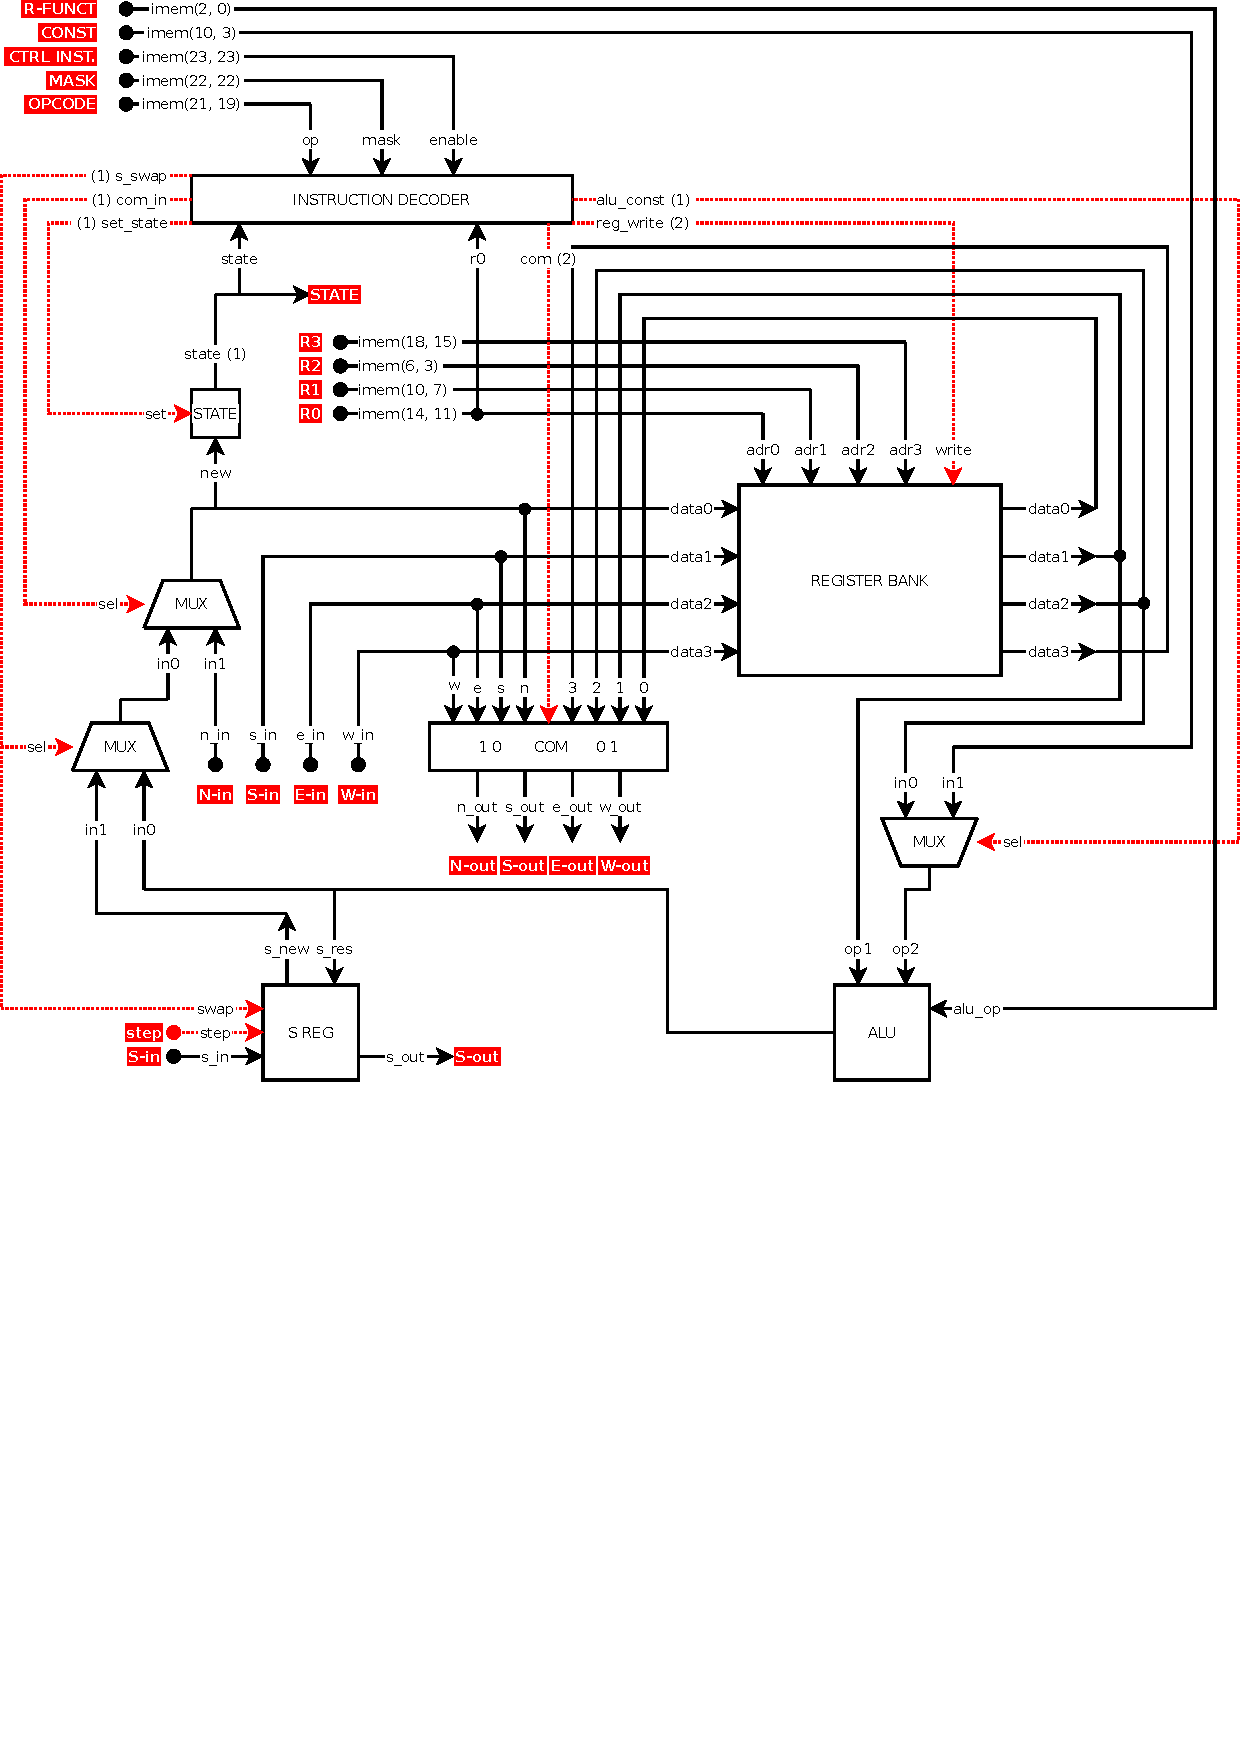
\includegraphics[width=\linewidth,clip,trim=0 0 0 0]
                  {fig/fpga/fpga-simd-arch.pdf}
  \caption{LENA SIMD architecture}
  \label{fig:fpga-simd-arch}
\end{figure}


\subsection{Components}
In order to the keep the signals to a minimum, the SIMD node is nicely divided
into separate components which makes up the datapath for the node.

\subsection{Instruction Decoder}
The instruction decoder is the control component of a node. It takes the opcode
of the instruction and sets control signals for all the other components in the
node.

\subsection{I/O Controller}

\subsection{Register Bank}

\subsection{ALU}

\subsection{S Register}
The source data register, S REG for short, is a special purpose register within
the SIMD node. S REG holds the next source data for the node. It is partly
controlled by the instruction set for the node and partly controlled by a
special {\tt step} signal from the DMA.

This register also has the capability to receive data from the left node,
through the {\tt s\_in}-bus, and passing it along to node on the right through
the {\tt s\_out}-bus when instructed by the {\tt step} signal. This allows a
simultaneous data transfer while the node is busy processing.

Rising the value on the {\tt swap} control signal will write the result from the
ALU to the S\_REG and copy the data from the S\_REG out to the {\tt s\_new} bus,
ultimately writing this data to the register bank.

\subsection{State Register}

\subsection{Registers}
Each SIMD node have $2^4 = 16$ general purpose registers. 4 of these are
available for general storage when executing instructions. The remaining 2
registers are the special purpose registers {\tt \$zero} and {\tt \$state}.

\begin{table}[h]
  \centering
  \begin{tabularx}{\linewidth}{XXXXXXXXX}\toprule
    R0 & R1 & R2 & R3 & R4 & R5 & R6 & R7 \\ \midrule
    \tt \$zero & \tt \$r1 & \tt \$r2 & \tt \$r3 & \tt \$r4 & \tt \$r5 &
    \tt \$r6 & \tt \$r7\\ \bottomrule
  \end{tabularx}
  \begin{tabularx}{\linewidth}{XXXXXXXX}
    R8 & R9 & R10 & R11 & R12 & R13 & R14 & R15 \\ \midrule
    \tt \$r8 & \tt \$r9 & \tt \$r10 & \tt \$r11 & \tt \$r12 & \tt \$r13 &
    \tt \$r14 & \tt \$state\\ \bottomrule
  \end{tabularx}
  \caption{Registers in the SIMD nodes}
  \label{tab:simd-registers}
\end{table}


\subsection{State-register}

\subsection{Zero-register}

\subsection{BRAM and SRAM}
BRAM or SRAM is not available from the SIMD node.

\subsection{Instruction Set}

\begin{figure}[h]
  \centering
  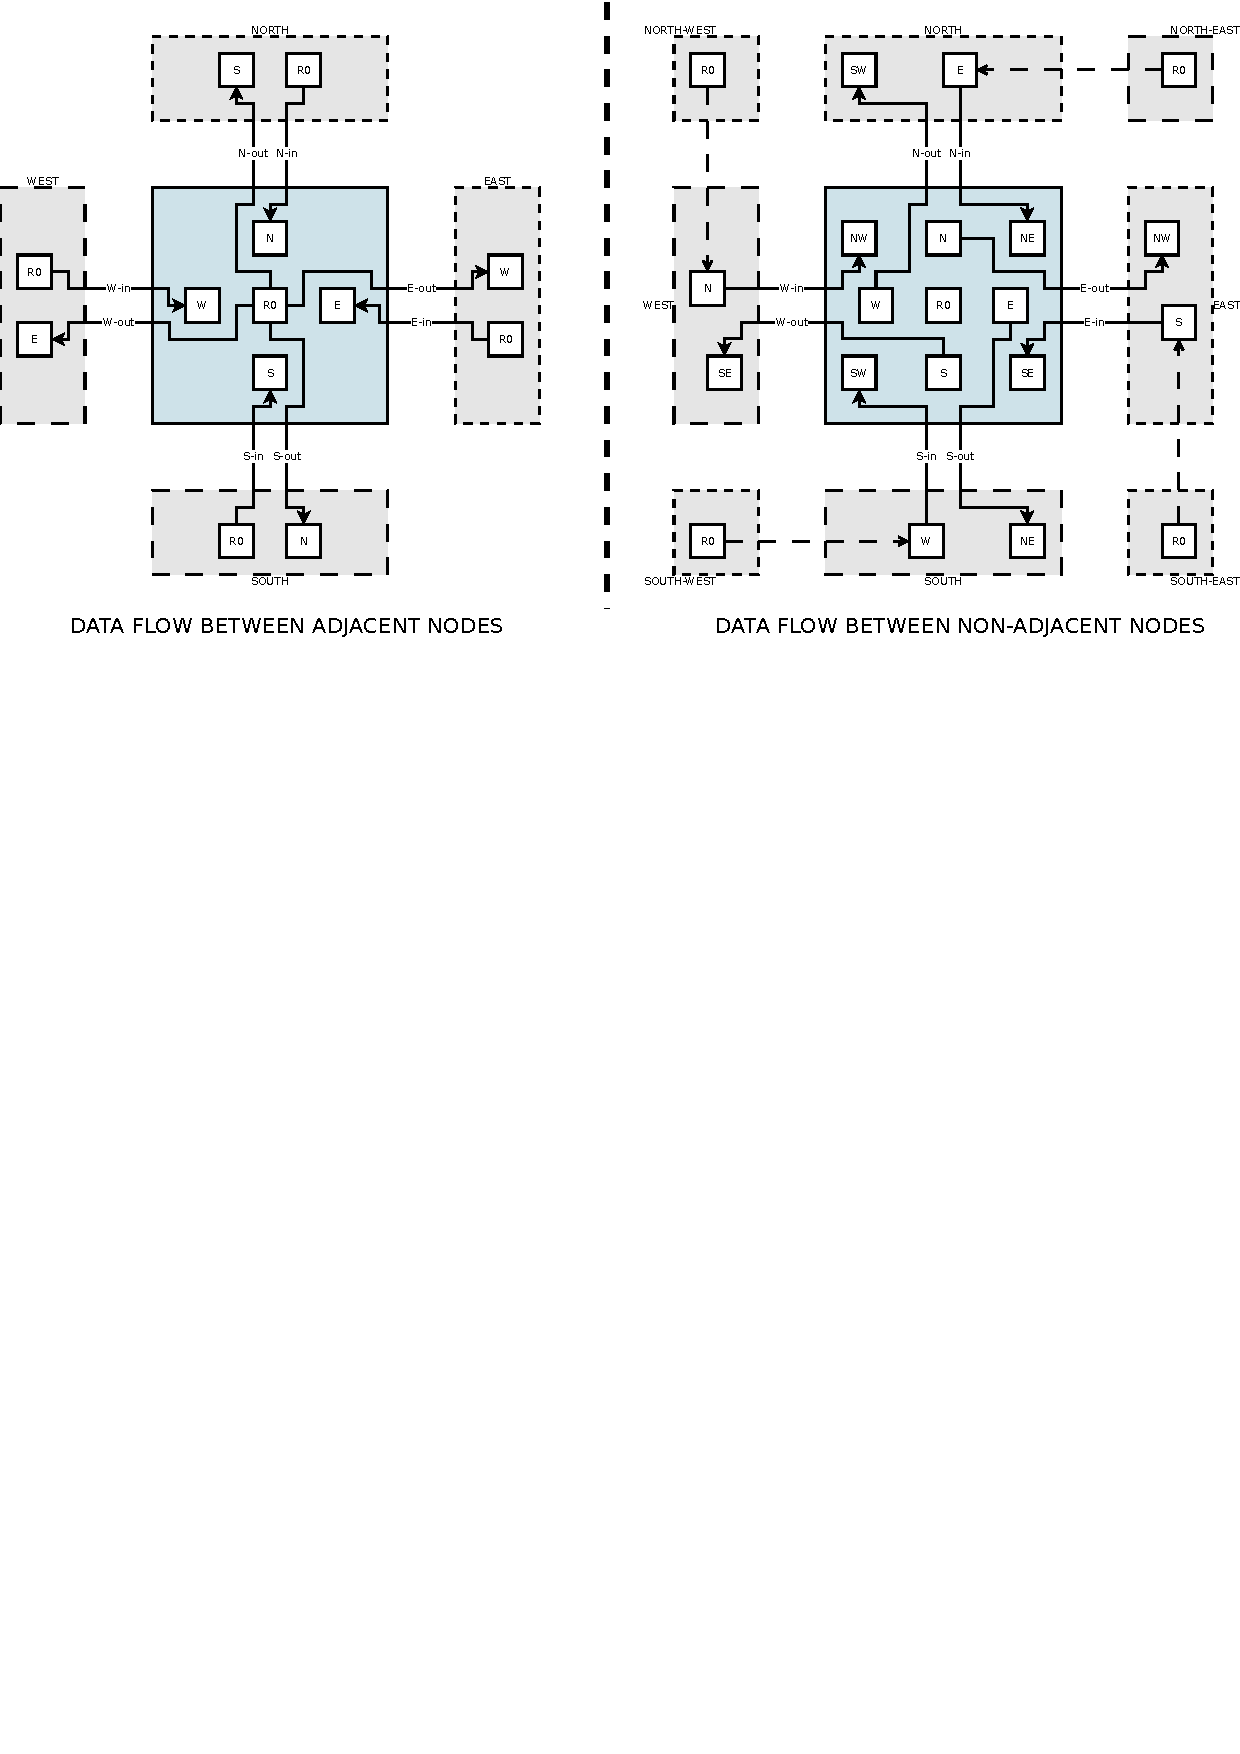
\includegraphics[width=\linewidth,clip,trim=0 18cm 0 0]
                  {fig/fpga/fpga-simd-datacom.pdf}
  \caption{Four-way communication in the LENA SIMD array.}
  \label{fig:fpga-simd-datacom}
\end{figure}



\subsection{Branching}
Since all nodes run the same instructions, both parts of a branch must be
executed. Nodes are setting the {\tt state} to 1 in order to indicate that they
are executing within that part of the branch.

\begin{table}[h]
  \centering
  \begin{tabularx}{\textwidth}{rlcX}\toprule
    \thxc{step} & \thxc{instruction} & \thxc{state} & \thxc{description} \\
    \midrule
    0 & \tt // initial state & 0 & \\
    1 & \tt eq \$state \$r1, \$r2 & 1
    & Set state to 1 if branch should be taken for the node.\\
    \ldots & \tt // branch taken & 1 &
    Instructions for when the branch is taken.\\
    2 & \tt eq \$state, \$state, \$zero & 0 & Negate the state.\\
    \ldots & \tt // branch not taken & 0 & Instructions for when the branch is
    not taken.\\ \bottomrule
  \end{tabularx}
  \caption{Single level branching}
  \label{tab:single-level-branching}
\end{table}


\subsection{Multilevel branching}
Since state register is 8 it is possible to have up-to 8 nested branches by
shifting the current state to the left and adding the new state to the
end. Below \TODO{Refer to table, not relative to where it is placed} are the
instructions for performing a multilevel-branch.

\CHECK{Better switch out zeroes and ones with x'es and y's?}
\begin{table}[h] % TODO: Drag out
  \centering
  \begin{tabularx}{\textwidth}{rlcX}\toprule
    \thxc{step} & \thxc{instruction} & \thxc{state} & \thxc{description} \\
    \midrule
    0 & \tt // initial state & 01 & \\
    1 & \tt sll \$r3, \$state & 01
    & Save the current state by shifting left.\\
    2 & \tt eq \$r4 \$r1, \$r2 & 01
    & Calculate if branch is taken for the node.\\
    3 & \tt add \$state \$r4, \$r3 & 11
    & Set the new state.\\
    \ldots & \tt // branch taken & 11 &
    Instructions for when the branch is taken.\\
    4 & \tt andi \$r3, \$state, 1111 1110 & 11
    & Save the old state for the node.\\
    5 & \tt andi \$r4, \$state, 0000 0001 & 11 & Save the current state.\\
    6 & \tt eq \$r4, \$r4, \$zero & 11 & Negate the current state.\\
    7 & \tt add \$state, \$r4, \$r3 & 10 & Set new state.\\
    \ldots & \tt // branch not taken & 10
    & Instructions for when the branch is not taken.\\
    8 & \tt srl \$state, \$state & 01 & Revert to state before branch by
    shifting right.\\ \bottomrule
  \end{tabularx}
  \caption{Multi level branching}
  \label{tab:multi-level-branching}
\end{table}

\CHECK{Could any of these tables be figures instead?}
